\chapter*{Chapter 4}

\section*{Section 4.2}
\begin{definition} [htb]
$AW: M \rightarrow ({\bigcup_{r\in R}r})^2$ \\ 
\caption{Change to def 4.2}
\label{def:config}
\end{definition}

$AW$ is a function, which for a module $m \in M$ returns the set of works, which $m$ performs activly on at least one recipe $r \in R$. $Start$ is a partial function, which maps a line $\gamma \in \Gamma$ to a module $m \in M$ such that $m \in \gamma'$ where $\gamma' \in \Gamma$ and $\gamma \neq \gamma'$. This represents that there is a vertical path between $m$ and the first element of $\gamma$. Similarly the partial function $End$, which maps a line $\gamma \in \Gamma$ to a module $m \in M$ such that $m \in \gamma'$ where $\gamma' \in \Gamma$ and $\gamma \neq \gamma'$. This represent that there is a vertical path from the last element of $\gamma$ to $m$.  

\[\texttt{if } \gamma \in \Gamma \cup \{\Gamma_0\} \texttt{ then } \forall m \in \gamma \land \forall \gamma ' \in \Gamma \land \gamma \neq \gamma ',\, m \notin \gamma ' \]

\[\texttt{if } m \in M \texttt{ then } AW(m) \subseteq m \land m \subseteq \bigcup_{r\in R}r\] 


\section*{Section 4.3}

\begin{definition}[htb]
\runatt{AS}{0}
    \infrule
        {0 < |B_{r,s,e}| \land |A_{r,s,e}| = |B_{r,s,e}| \land  s <_k e}
        {(R,M,\Gamma, \Gamma_0, AW, Start, End) \rightarrow_{AS}
        (R,M,\Gamma', \Gamma_0', AW, Start', End') } \\
        Where: \\
        $r \in R$ \\
		$s,e \in K_{\Gamma_0,r}$\\		
		$\Gamma_0' = (Pre_s \cup \{s\}  \cup A_{r,s,e} \cup \{e\} \cup Pos_e, \prec)$ \\     
        $\Gamma' = \Gamma \cup B_{r,s,e} $ \\
		$Start' = Start \cup \{(B_{r,s,e}, s)\}$ \\
		$End' = End \cup \{(B_{r,s,e}, e)\}$

\caption{Formal definition of the $AS_0$ transformation rule}
\label{def:as0}
\end{definition}

\[a <_K b = \left\{\begin{matrix}
tt \texttt{ if } a,b \in K_{\Gamma_0 ,r} \land a \prec b \land \nexists c \in K_{\Gamma_0 ,r}, c \neq a \land c \neq b \land a \prec c \land c \prec b \\ \texttt{else } ff
\end{matrix}\right.\]

We also define a totally ordered set of all modules in between two modules, $s$ and $e$, in some line $\gamma \in \Gamma \cup \{\Gamma_0\} $:

\[M_{s,e} = (\{m | m \in \gamma \land \gamma \in \Gamma \cup \{\Gamma_0\} \land s \prec m \land m \prec e\}, \prec)\]

We can now define the totally ordered set of all modules appearing between $s$ and $e$, which are not used to work $r$, $A_{r,s,e}$ as follows: 

\[A_{r,s,e} = (\{m |m \in M_{s,e} \land m \in \alpha\}, \prec)\]

Similarly we can define the totally ordered set $B_{r,s,e}$, which contains all modules that appear between $s$ and $e$ which work exclusively on $r$

\[B_{r,s,e} = (\{m |m \in M_{s,e} \land m \in \beta\}, \prec)\]

We define $Pre_{s}$ which is the totally ordered set of all modules that come before a module $s$ in line $\gamma \in \Gamma$:
\[Pre_{s} = (\{m | m \in \gamma \land \gamma \in \Gamma \land m \prec s\}, \prec)\]

And lastly we define $Pos_{e}$ which is the totally ordered set of all modules that come after a module $e$  in line $\gamma \in \Gamma$:
\[Pos_{e} = (\{m | m \in \gamma \land \gamma \in \Gamma \land e \prec  m \}, \prec)\]

Having defined these totally ordered sets the rule in \cref{def:as0}, shows that in the case where $|B_{r,s,e}| > 0 \land s <_K e$ then we may update $\Gamma$ with a new lines defined by the total order $B_{r,s,e}$ in addition to an update of $\Gamma_0$, which removes $B_{r,s,e}$ from the line. This describes a branch out from $\Gamma_0'$, which exclusively works upon $r$ before rejoining with the old line. 

\begin{figure}[H]
\centering
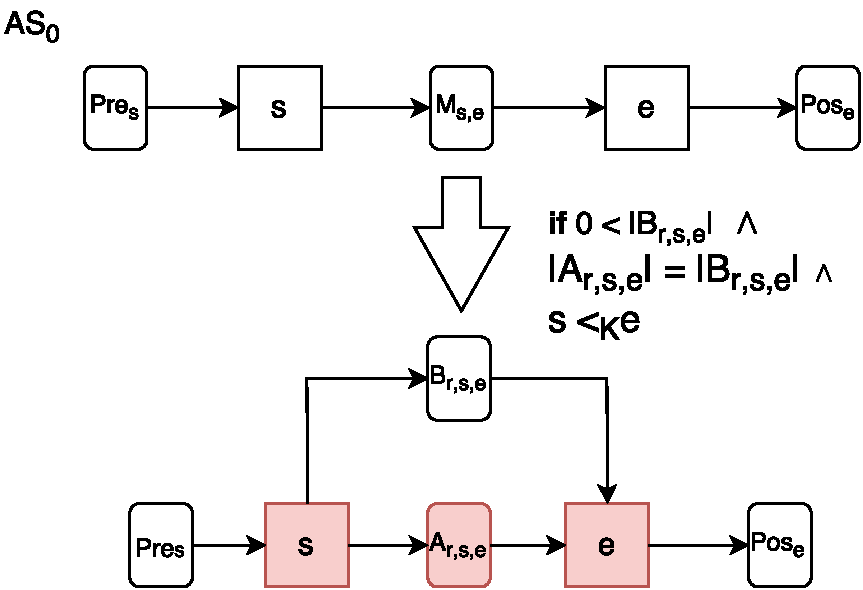
\includegraphics[width=\textwidth]{as0.pdf}
\caption{A visual representation of the $AS_0$ transformation rule}
\label{fig:as0}
\end{figure}

\section*{Section 4.4}
\[ParaMapPaths_{X} = \{p \in ParaMap_{X}^2 | (m,m') \in p \land (n,n') \in p \land |p| = |X| \land  \forall m': m' \neq n' \land  \forall m: m \neq n \}\]

\section*{Section 4.5}
\[AW' = (AW \cup \{(b, AW(a))\}) \setminus \{(a, AW(a))\}\]

\[AW' = (AW \cup \{(b, AW(a)), (a, AW(b)\}) \setminus \{(a, AW(a)), (b, AW(b))\}\]

